\chapter{Experiments}

This chapter will cover the experiments implemented throughout this project, which focused on reducing data sets with the presented algorithms and evaluating these reductions. Once again, it is quite difficult to evaluate reductions, but a set of metrics were adopted to attempt to understand them as much as possible. All experiments follow the format bellow:

Let $X_{n \times f}$ be a data set with $n$ samples and $f$ features, and $D \subset \mathbb{N} \mid d \in D \implies d \le f$ a  set of dimensions to which $X$ should be reduced.

\begin{enumerate}
	\item The data set $X$ is loaded and its first three features are plotted, given an initial idea of how the data is distributed for those features.
	\item $X$ is reduced to 3, 2 and 1 dimensions. Each reduction is plotted for visualization.
	\item Kruskal's stress is calculated for $X$.
	\item A 1-NN classifier or regressor is trained with 80\% of $X$'s samples and tested with the other 20\%. The score is kept for future reference.
	%TODO Talk about r2_score and class_score.
	\item Grid search is executed over $X$ using a SVM classifier or regressor. This step evaluates how a ``real world" algorithm would perform over the original data set.
	\item for $d \in D$:
	\begin{enumerate}
		\item $X$ is embbeded into the $\mathbb{R}^d$, creating the data set $Y_{n \times d}$.
		\item Kruskal's stress is calculated for $Y$.
		\item A 1-NN classifier or regressor is trained with the same samples used in step 4, and tested with all the others. The score is compared to the one retrieved in step 4.
		\item Grid Search is executed over $Y$ and the score is compared to the one presented in step 5.
	\end{enumerate}
\end{enumerate}

\section{Classification and Regression Over Linearly Reduced Data Sets}
\label{sec:experiments_linear_ds}

\subsection{$K$ Data Set}

The figure bellow illustrates the results of PCA algorithm application over the artificial $K$ data set. Notice that, for the second application, it correctly chose to discard the vertical dimension, as the samples offer less variability in this component.

\begin{figure}[H]
	\centering
	\captionsetup{justification=centering}
	
	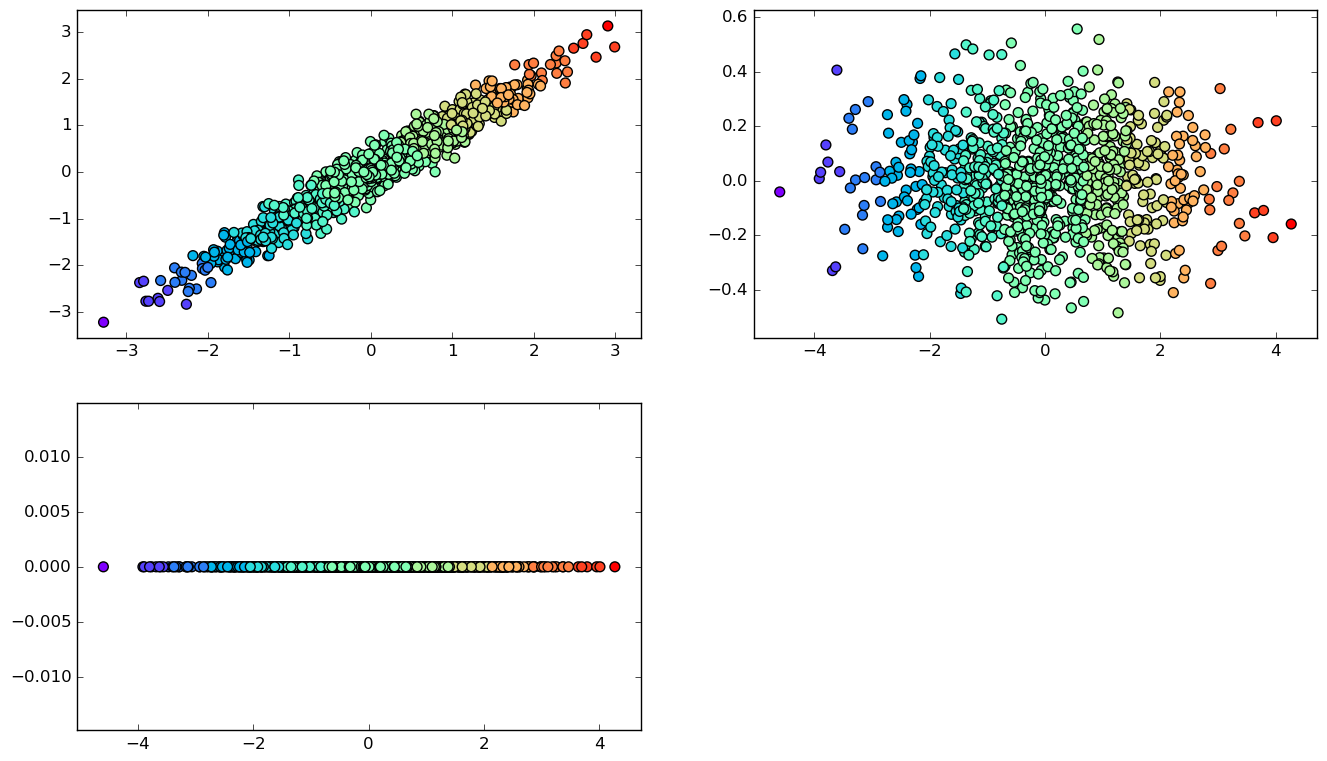
\includegraphics[width=.9\linewidth]{experiments/pca_r}
	\caption{The PCA algorithm reducing $K$ to 2 and 1 dimension, respectively.}
	\label{fig:datasetrpca}
\end{figure}

\begin{table}[H]
	\centering
	\begin{tabular}{|c|c|c|c|}
		\hline
		& \textbf{Original $\mathbb{R^2}$} & \textbf{$\mathbb{R}^2$} & \textbf{$\mathbb{R}$} \\\hline
		\textbf{Pred. accuracy} & .98 & .98 & .99 \\\hline
		\textbf{GridSearch time} & 1.15 s & .84 s & 1.26 s \\\hline
		\textbf{Reduction time} & - & 0.995 ms & 1.118 ms \\\hline
		\textbf{Stress} & - & 0 & .0399 \\\hline
		\textbf{Data size} & 15.62 KB & 15.62 KB & 7.81 KB \\\hline
	\end{tabular}
	\caption{Description of predictions and reduction performance for $K$.}
\end{table}

From the table above, one can also observe how Kruskal's stress might not be an appropriate quality measurement, given a specific domain. Indeed, for data set $K$, stress increase resulted from the removal of one of the components did not imply on prediction accuracy decrease.

\clearpage
\subsection{The Iris Flower Data Set}

The Iris flower from section \ref{irisdataset}, containing 150 samples and 5 features.

\begin{figure}[H]
	\centering
	\captionsetup{justification=centering}
	
	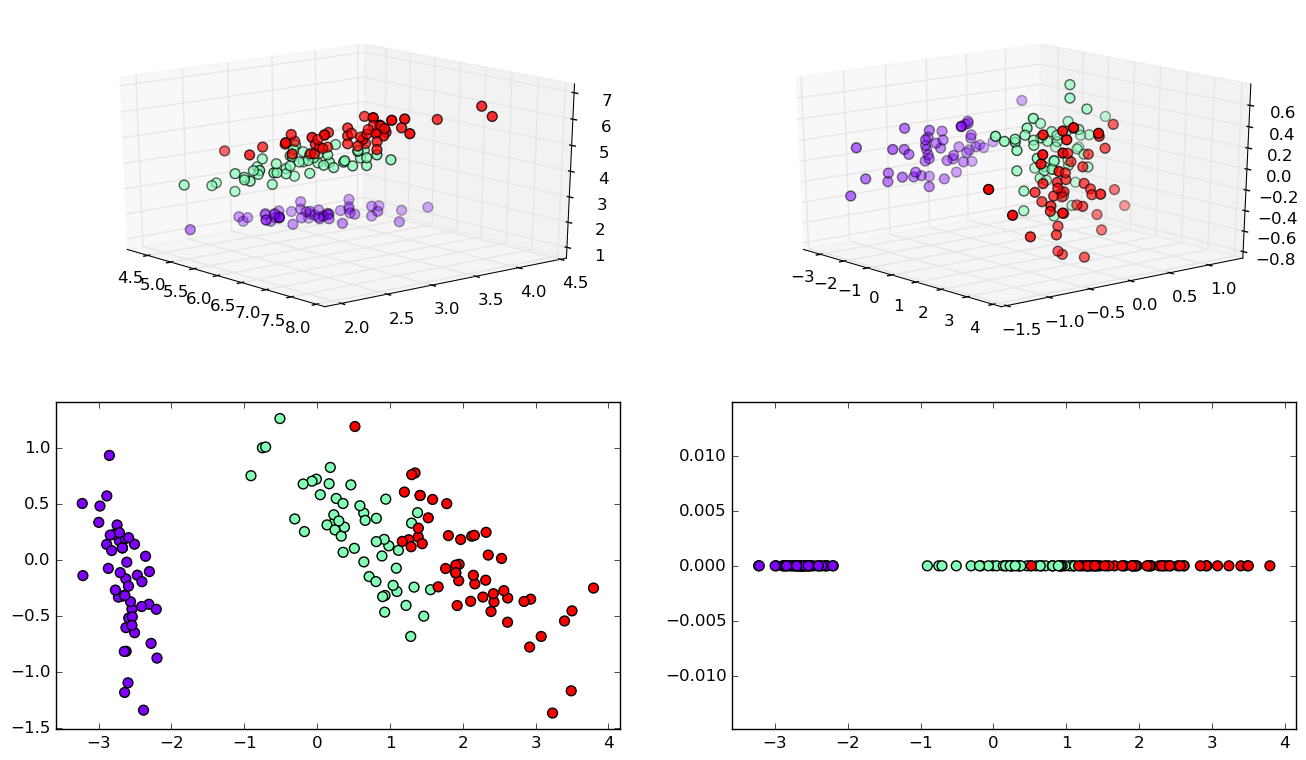
\includegraphics[width=\linewidth]{experiments/pca_iris}
	\caption{The Iris Flower data set and its reductions to 3, 2, and 1 dimensions, respectively.}
	\label{fig:dsirispca}
\end{figure}

Although the data set became nonlinearly separable, classes are still somewhat organized in different clusters.

\begin{table}[H]
	\centering
	
	\begin{tabular}{|c|c|c|c|}
		\hline
		& \textbf{Original data} & \textbf{Reduced data ($\mathbb{R}^2$)} & \textbf{Reduced data ($\mathbb{R}$)} \\\hline
		\textbf{Pred. accuracy} & .99 & .97 & .94 \\\hline
		\textbf{GridSearch time} & 1.71 s & 1.64 s & 1.78 s \\\hline
		\textbf{Reduction time} & - & 0.995 ms & 1.118 ms \\\hline
		\textbf{Stress} & - & .0418 & .1095 \\\hline
		\textbf{Data size} & 4.68 KB & 2.34 KB & 1.17 KB \\\hline
	\end{tabular}
	
	\caption{Description of predictions and reduction performance for Iris flower.}
\end{table}

\clearpage
\subsection{The Digits Data Set}

Digits data set is composed by 1797 samples, 64 features and 10 classes. Each sample is a 8x8 image of a hand-written digit from 0 to 9.

\begin{figure}[H]
	\centering
	\captionsetup{justification=centering}
	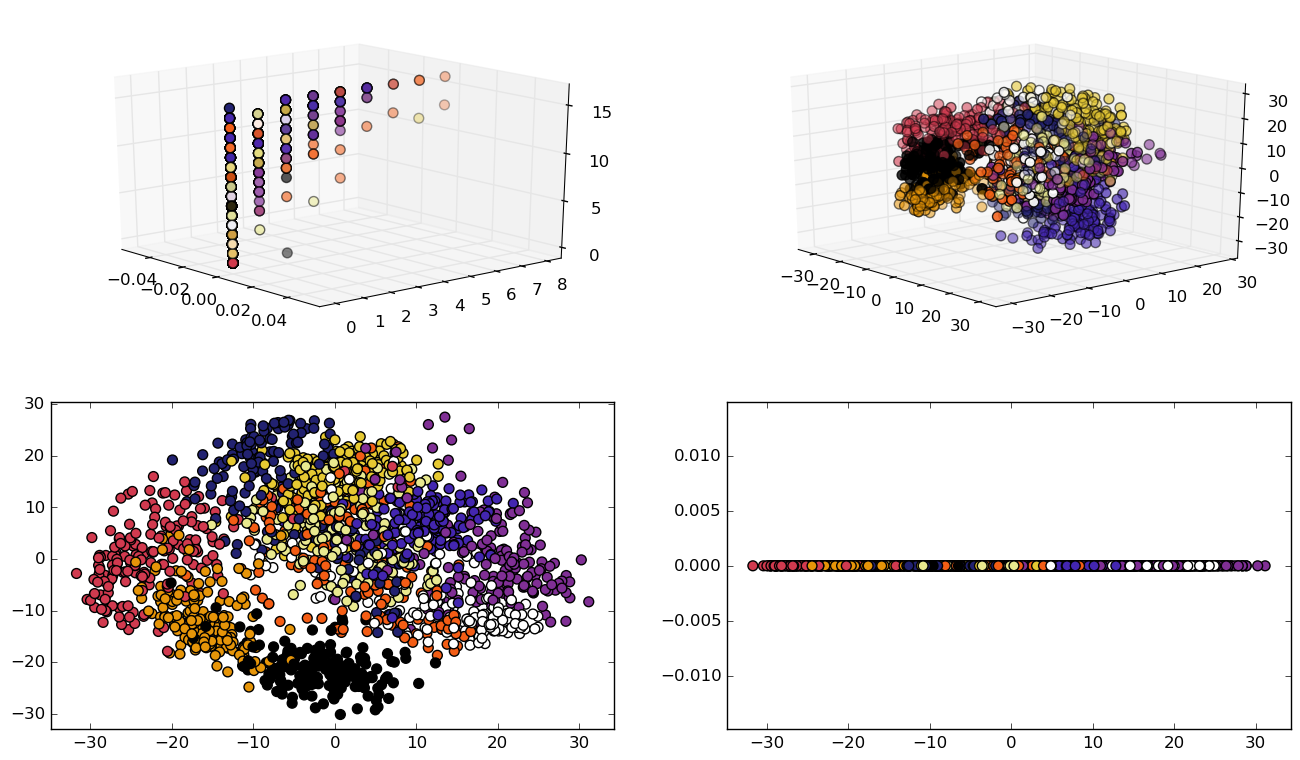
\includegraphics[width=\linewidth]{experiments/pca_digits}
	\caption{Digits data set reduced to 10, 3, 2 and 1 dimension, respectively.}
	\label{fig:dsdigitspca}
\end{figure}

\begin{table}[H]
	\centering
	\begin{tabular}{|c|c|c|c|c|c|}
		\hline
		& \textbf{$\mathbb{R}^{64}$} & \textbf{$\mathbb{R}^{10}$} & \textbf{$\mathbb{R}^3$} & \textbf{$\mathbb{R}^2$} & \textbf{$\mathbb{R}$} \\\hline
		\textbf{Pred. accuracy}   & .98 & .95 & .74 & .64 & .39 \\\hline
		\textbf{GridSearch time} & 8.51 s & 21.33 s & 151.04 s & 132.18 s & 113.78 s \\\hline
		\textbf{Reduction time} & - & 0.02 s & 0.01 s & 0.01 s & 0.01 s \\\hline
		\textbf{Stress} & - & .1594 & .4218 & .5405 & .7092 \\\hline
		\textbf{Data size} & 898.5 KB & 140.39 KB & 42.11 KB & 28.07 KB & 14.03 KB \\\hline
	\end{tabular}
	
	\caption{Description of predictions and reduction performance for Digits.}
\end{table}

Notice that it was possible to eliminate 54 dimensions, consistently reducing the data set size, and only suffering 3\% of prediction accuracy loss. The score drastically decreased, however, when more dimensions were removed. Furthermore, accuracy decrease was followed by stress increase.

\section{Classification and Regression Over Data Sets Reduced with ISOMAP}

Just as in \ref{sec:experiments_linear_ds}, this section reports reduction, classification and regression experiments made in common data sets, following the same format as before.

\subsection{The Swiss Roll Data Set}

\begin{figure}[H]
	\centering
	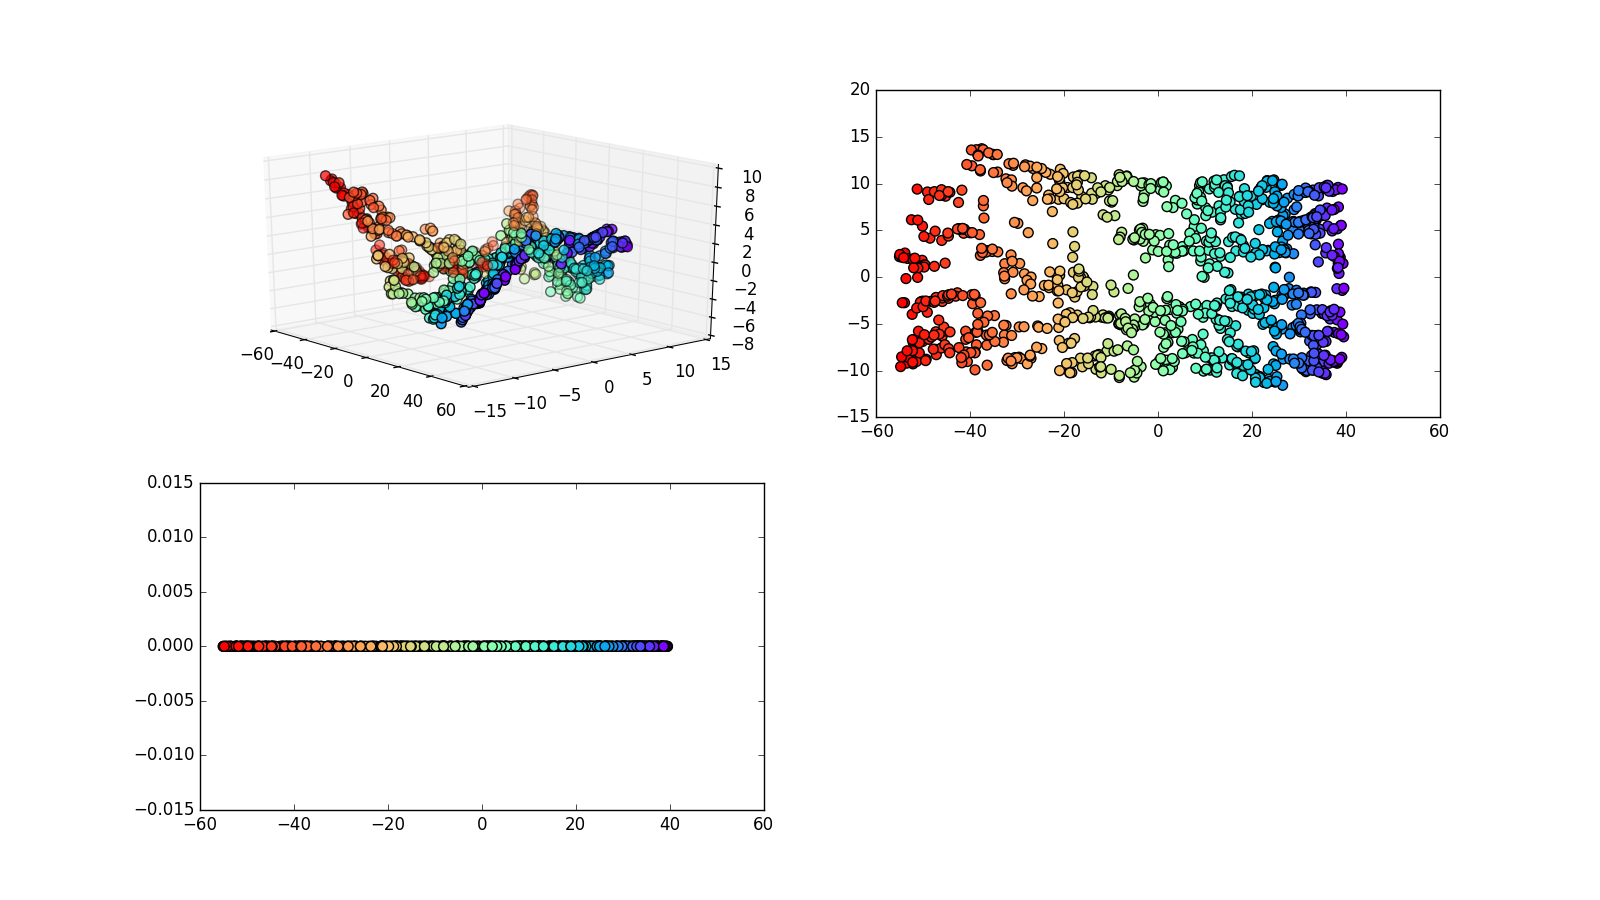
\includegraphics[width=.95\linewidth]{experiments/iso_swiss}
	\captionsetup{justification=centering}
	\caption{The Swiss Roll data set and its reductions to 2 and 1 dimensions, respectively.}
\end{figure}

\begin{table}[H]
	\centering
	\begin{tabular}{|c|c|c|c|}
		\hline
		& \textbf{Orig. $\mathbb{R}^3$} & \textbf{$\mathbb{R}^2$} & \textbf{$\mathbb{R}$} \\\hline
		\textbf{Prediction accuracy}   & 1            & 1             & 1     \\\hline
		\textbf{GridSearch time} & 15.53 s   & 415.72 s  & 387.98 s  \\\hline
		\textbf{Reduction time}  & -         & 0.51 s       & 0.48 s     \\\hline
		\textbf{Data size}          & 23.44 KB & 15.62 KB  & 7.81 KB   \\\hline
	\end{tabular}
	
	\caption{Description of predictions and reduction performance for Swiss Roll.}
\end{table}

\subsection{The Iris Flower Data Set}

Once again, the Iris flower data set, containing 150 samples and 5 features.

\begin{figure}[H]
	\centering
	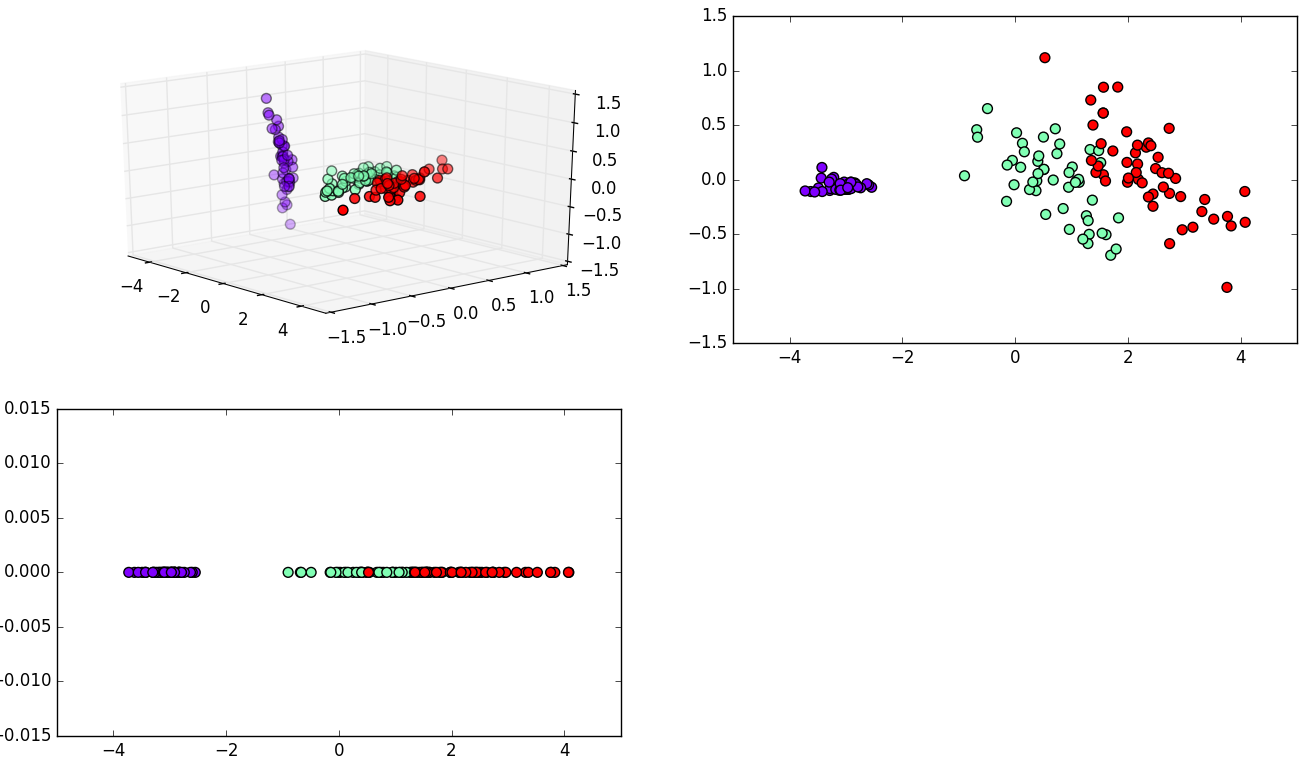
\includegraphics[width=\linewidth]{experiments/iso_iris}
	\captionsetup{justification=centering}
	\caption{The Iris data set and its reductions to 3, 2 an 1 dimensions, respectively.}
\end{figure}

\begin{table}[H]
	\centering
	\begin{tabular}{|c|c|c|c|c|}
		\hline
		& \textbf{Orig. $\mathbb{R}^4$} & \textbf{$\mathbb{R}^3$} & \textbf{$\mathbb{R}^2$} & \textbf{$\mathbb{R}$} \\\hline
		\textbf{Prediction accuracy}   & .99      & .97  s             & .97             & .89           \\\hline
		\textbf{GridSearch time}           & .27 s   & .25 s              & .25 s         & .27 s        \\\hline
		\textbf{Reduction time}             & -           & .19 s              & .19 s          & .36 s        \\\hline
		\textbf{Stress}                                  & -           & .474525      & .569293   & .655614 \\\hline
		\textbf{Data size}                           & 4.69 KB & 3.52 KB  & 2.34 KB   & 1.17 KB  \\\hline
	\end{tabular}
	
	\caption{Description of predictions and reduction performance for Iris.}
\end{table}

\newpage
\subsection{The Glass Data Set}

The Glass data set contains 214 samples and 11 features, were the first one is the identification number of a given sample and the last one is the class to which that sample belongs.

\begin{figure}[H]
	\centering
	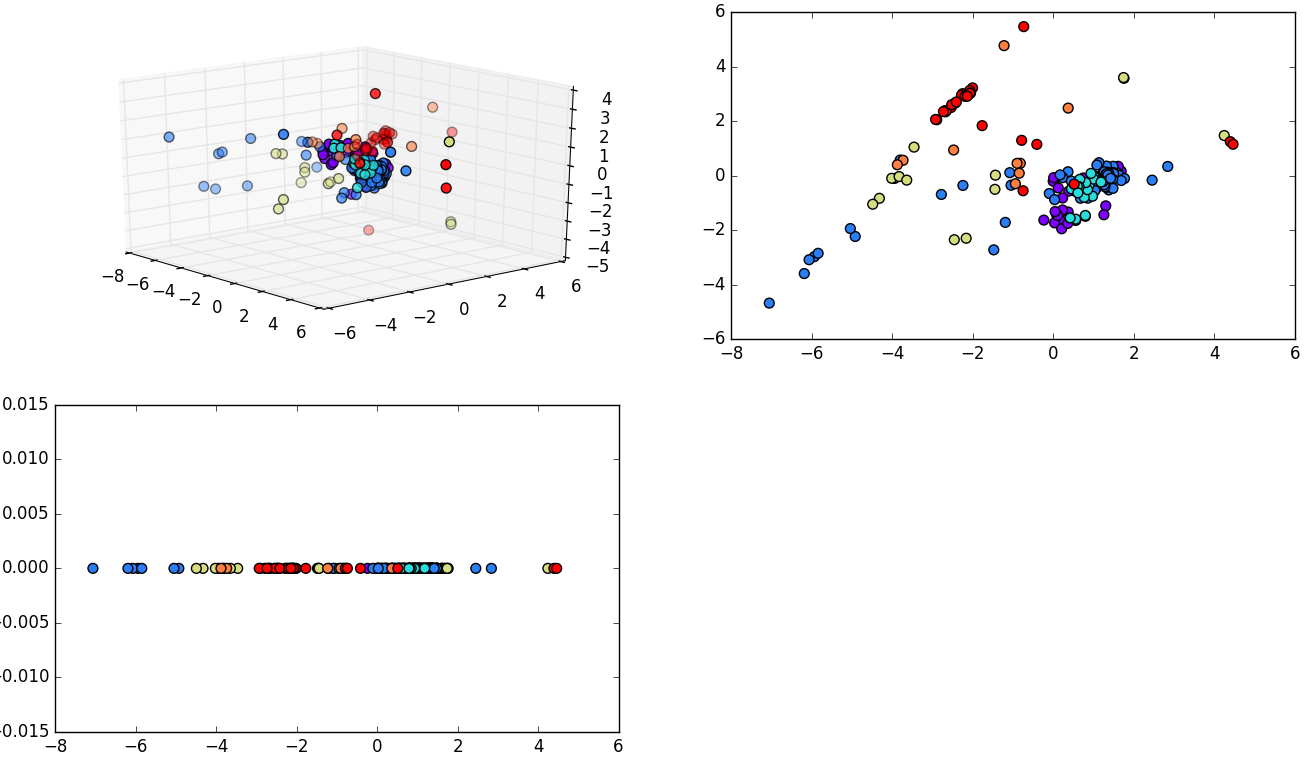
\includegraphics[width=\linewidth]{experiments/iso_glass}
	\captionsetup{justification=centering}
	\caption{The Glass data set and its reductions to 3, 2 an 1 dimensions, respectively.}
\end{figure}

\begin{table}[H]
	\centering
	\begin{tabular}{|c|c|c|c|c|c|}
		\hline
		& \textbf{Orig. $\mathbb{R}^{9}$} & \textbf{$\mathbb{R}^8$} & \textbf{$\mathbb{R}^6$} & \textbf{$\mathbb{R}^4$}  & \textbf{$\mathbb{R}^3$} \\\hline
		\textbf{Prediction accuracy}   & .64 & .63  & .66 & .65  & .65 \\\hline
		\textbf{GridSearch time} & .36 s & .35 s   & 2.77 s & 2.36 s & 1.26 s  \\\hline
		\textbf{Reduction time}  & -  & .66 s & .65 s & .68 s    & .64 s     \\\hline
		\textbf{Stress} & - & .513717 & .462840 & .362030 & .306092 \\\hline
		\textbf{Data size}          & 15.05 KB & 13.37 KB & 10.03 KB & 6.69 KB & 5.02 KB   \\\hline
	\end{tabular}
	
	\caption{Description of predictions and reduction performance for Glass.}
\end{table}

\newpage
\subsection{The Digits Data Set}

\begin{figure}[H]
	\centering
	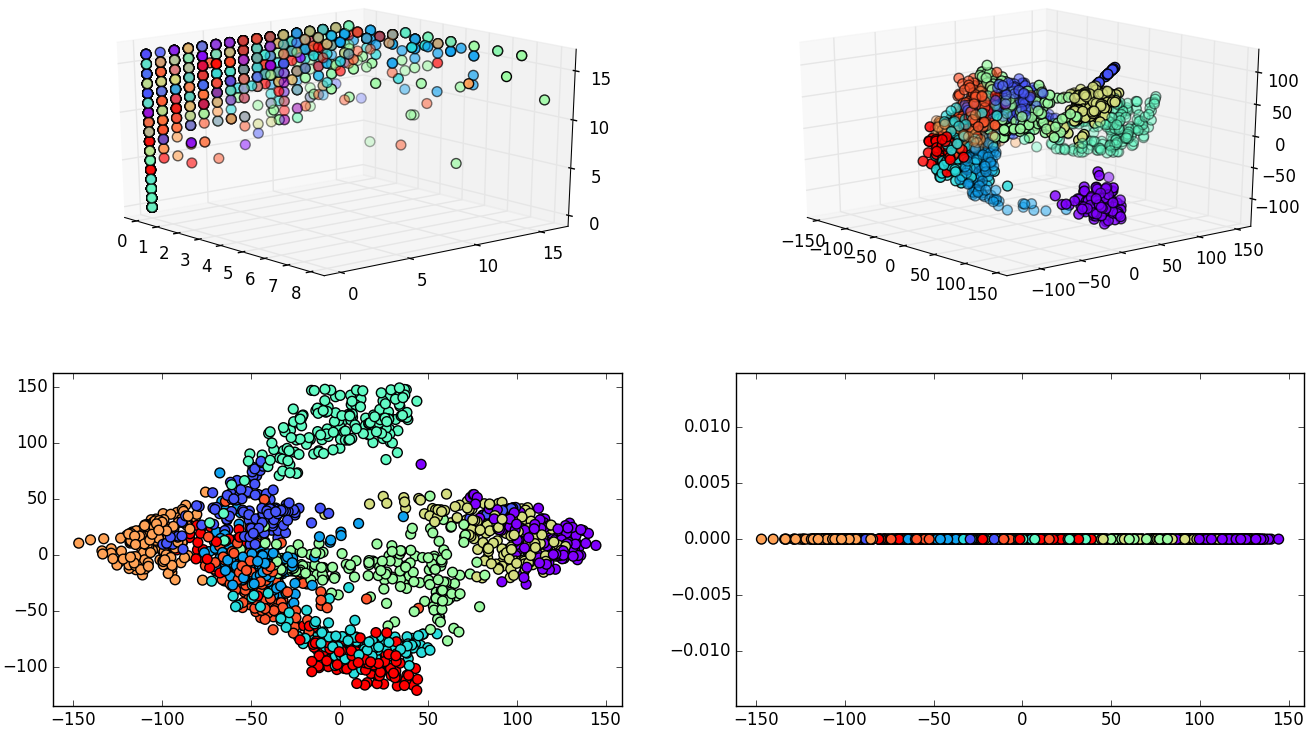
\includegraphics[width=\linewidth]{experiments/iso_digits}
	\captionsetup{justification=centering}
	\caption{Digits data set and its reductions to 3, 2 and 1 dimension, respectively.}
	\label{fig:dsdigitsiso}
\end{figure}

\begin{table}[H]
	\centering
	\begin{tabular}{|c|c|c|c|c|c|}
		\hline
		& \textbf{Orig. $\mathbb{R}^{64}$} & \textbf{$\mathbb{R}^{10}$} & \textbf{$\mathbb{R}^3$} & \textbf{$\mathbb{R}^2$} & \textbf{$\mathbb{R}$} \\\hline
		\textbf{Pred. accuracy}   & .98 & .96 & .91 & .69 & .45 \\\hline
		\textbf{GridSearch time} & 12.22 s & 98.08 s & 287.46 s & 630.47 s & 949.88 s \\\hline
		\textbf{Reduction time}  & - & 5.43 s & 2.72 s & 2.71 s & 2.04 s \\\hline
		\textbf{Data size} & 898.50 KB & 140.39 KB & 42.12 KB & 28.08 KB & 14.04 KB \\\hline
	\end{tabular}
	
	\caption{Description of predictions and reduction performance for Digits.}
\end{table}

Notice that the data set was reduced to only 3 dimensions, while maintaining 91\% of accuracy (remember that dimensionality reduction with PCA would reduce accuracy to 74\%). Accuracy loss is still observable when reducing it to two or one dimensions, although it is less intense than losses caused by linear reduction.

\newpage
\subsection{The Dermatology Data Set}

The Dermatology data set, composed by 366 samples and 35 features. Here, the target is to correctly diagnose the erythemato-squamous diseases.

\begin{figure}[H]
	\centering
	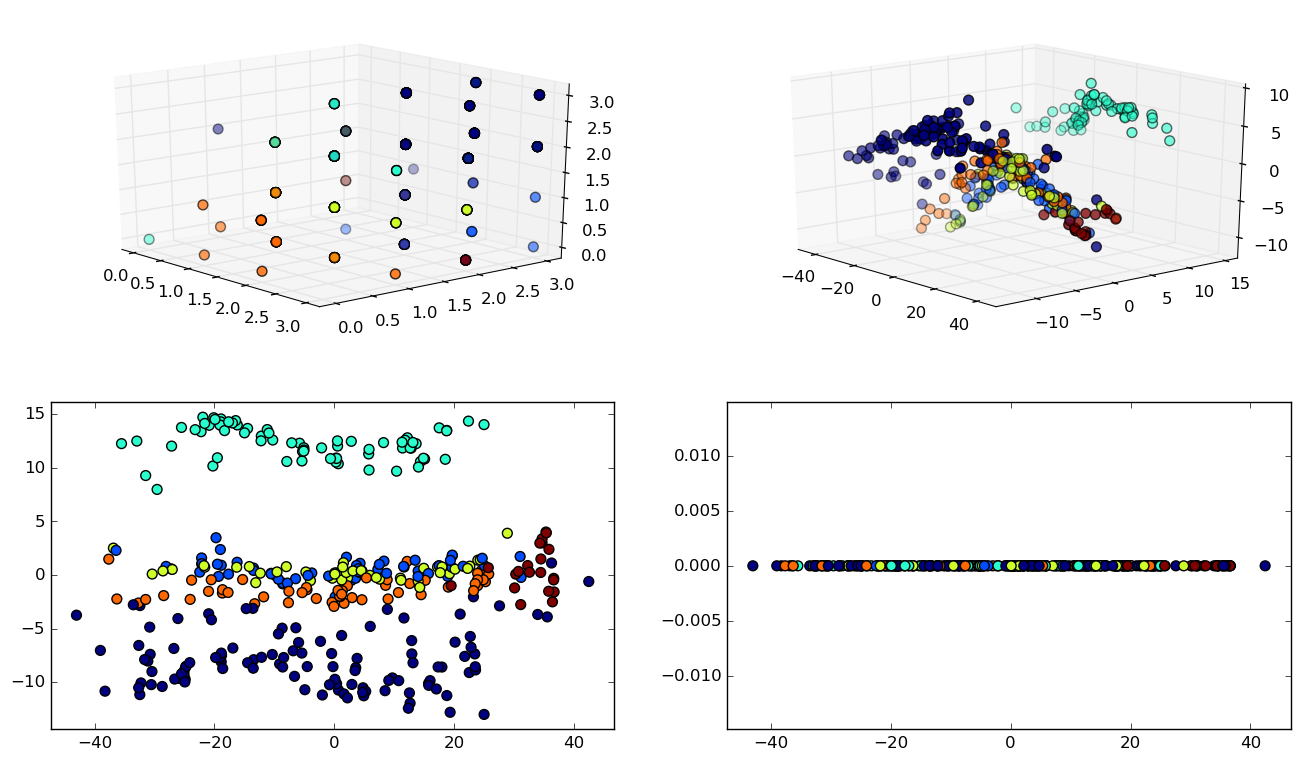
\includegraphics[width=\linewidth]{experiments/iso_dermatology}
	\captionsetup{justification=centering}
	\caption{The Dermatology data set and its reductions to 3, 2 an 1 dimensions, respectively.}
\end{figure}

\begin{table}[H]
	\centering
	\begin{tabular}{|c|c|c|c|c|c|}
		\hline
		& \textbf{Orig. $\mathbb{R}^{34}$} & \textbf{$\mathbb{R}^{20}$} & \textbf{$\mathbb{R}^{10}$} & \textbf{$\mathbb{R}^3$} & \textbf{$\mathbb{R}^2$} \\\hline
		\textbf{Prediction accuracy}  & .953552 & .915301 & .907104 & .827869 & .784153 \\\hline
		\textbf{GridSearch time} & .67 s & .76 s & 2.06 s & 27 s & 44.1 s  \\\hline
		\textbf{Reduction time}  & -         & 5.1 s & 4.89 s & 4.91 s & 4.96 s    \\\hline
		\textbf{Stress} & - & .771817 & .597724 & .465458 & .416376 \\\hline
		\textbf{Data size}          & 97.22 KB & 57.19 KB & 28.59 KB  & 8.59 KB & 5.72 KB  \\\hline
	\end{tabular}
	
	\caption{Description of predictions and reduction performance for Dermatology.}
\end{table}

\newpage
\subsection{The Leukemia Data Set}

Extracted from \href{http://mldata.com}{mldata}, the Leukemia data set contains 72 samples and 7130 features. The first 7129 features are expression levels of the genes in a given patient. The 7130th feature $t \in \{-1, 1\}$ indicate which of two variants of leukemia is present in the sample (AML, 25 samples, or ALL, 47 samples). \cite{on:duc_ds}

The Results in this experiment are quite impressive: although visualization has barely changed from 7129 to 3 dimensions, a 7129-dimensional space was reduced to a 10-dimensional one with only 10\% of accuracy loss.

\begin{figure}[H]
	\centering
	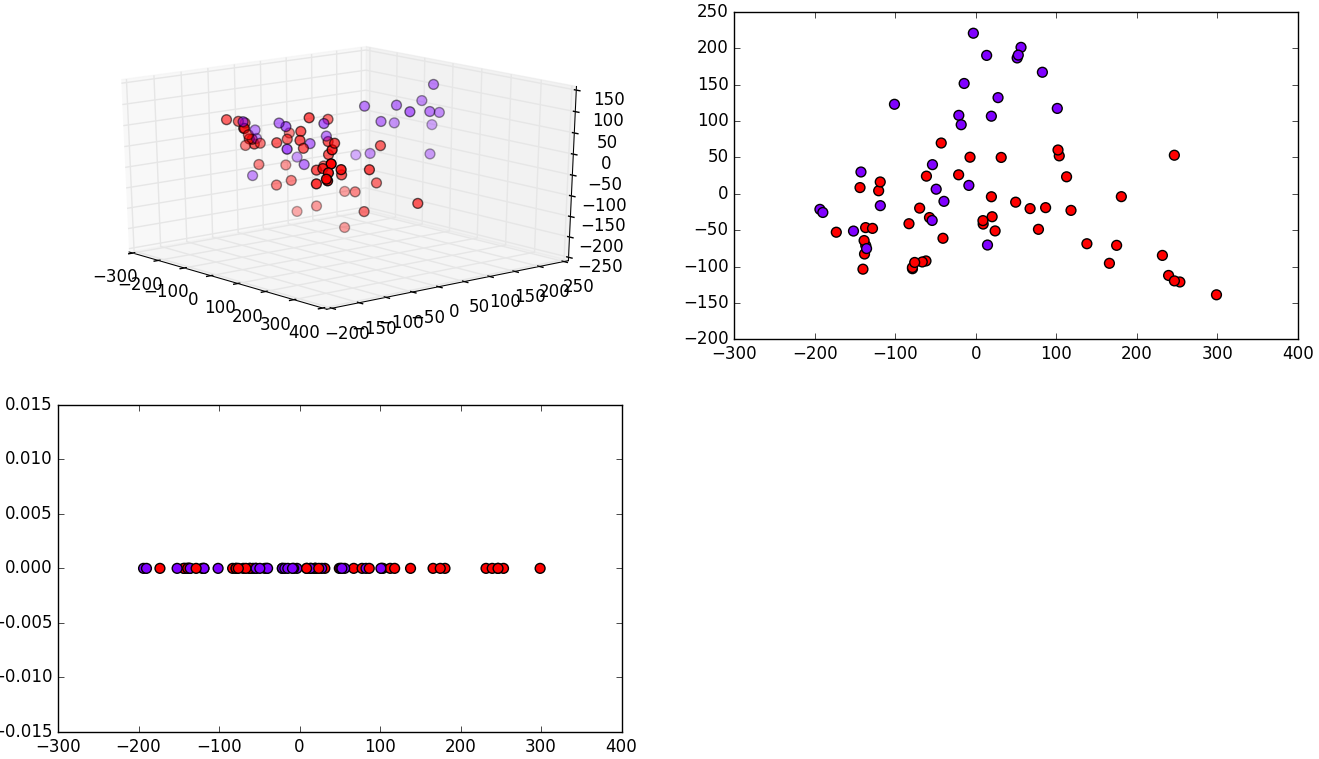
\includegraphics[width=.9\linewidth]{img/experiments/iso_leukemia}
	\captionsetup{justification=centering}
	\caption{The Leukemia data set and its reduction to 3, 2 and 1 dimensions, respectively.}
	\label{fig:leukemiads}
\end{figure}

\begin{table}[H]
	\centering
	\begin{tabular}{|c|c|c|c|c|}
		\hline
		& \textbf{Orig. $\mathbb{R}^{7129}$} & \textbf{$\mathbb{R}^{30}$} & \textbf{$\mathbb{R}^{20}$} & \textbf{$\mathbb{R}^{10}$} \\\hline
		\textbf{Pred. accuracy}    & .99 & .88 & .85 & .88 \\\hline
		\textbf{GridSearch time}   & 2.42 s & .26 s & .26 s & 141.13 s \\\hline
		\textbf{Reduction time}    & - & .06 s & .04 s & .04 s \\\hline
		\textbf{Data size}         & 4010.06 KB & 16.88 KB & 11.25 KB & 5.62 KB \\\hline
	\end{tabular}
	\captionsetup{justification=centering}
	\caption{Description of predictions and reduction performance for Leukemia data set.}
\end{table}

\subsection{The WDBC Data Set}

The Wisconsin Diagnostic Breast Cancer (WDBC) data set, containing 596 samples and 32 features computed from a breast mass. WDBC has benign 357 samples and 212 malignant. During this experiment, the first feature was disregarded, as it represents the identification numbers of the samples.

Regarding the experiment, observe how prediction accuracy consistently increased when the data set was reduced.

\begin{figure}[H]
	\centering
	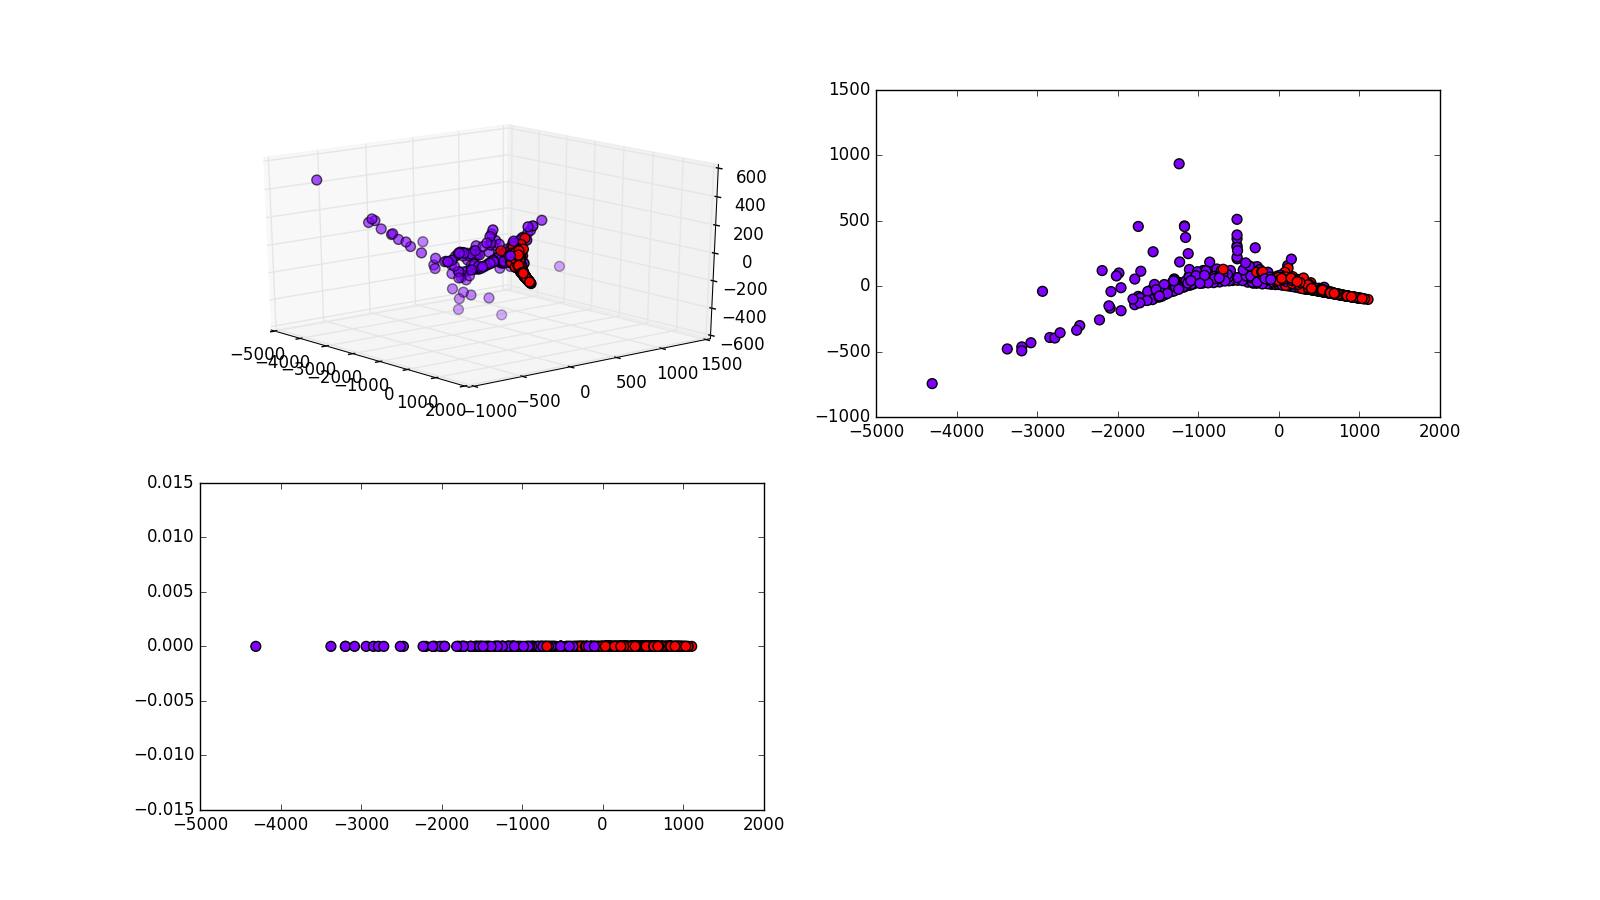
\includegraphics[width=.9\linewidth]{img/experiments/iso_wdbc}
	\captionsetup{justification=centering}
	\caption{The WDBC data set and its reduction to 3, 2 and 1 dimensions, respectively.}
	\label{fig:iso_wdbc}
\end{figure}

\begin{table}[H]
	\centering
	\begin{tabular}{|c|c|c|c|c|c|}
		\hline
		& \textbf{Orig. $\mathbb{R}^{30}$} & \textbf{$\mathbb{R}^{20}$} & \textbf{$\mathbb{R}^{10}$} & \textbf{$\mathbb{R}^{3}$} & \textbf{$\mathbb{R}^{2}$} \\\hline
		\textbf{Pred. accuracy}    & .63 & .89 & .8963 & .8998  & .8998 \\\hline
		\textbf{GridSearch time}   & 0.58 s & 0.46 s & 0.36 s & 0.36 s & 0.36 s \\\hline
		\textbf{Reduction time}    & - & 3.31 s & 3.25 s & 3.26 s & 3.31 s \\\hline
		\textbf{Stress} & - & .53 & .465460 & .378905 & .352277 \\\hline
		\textbf{Data size}  & 133.36 KB & 88.91 KB & 44.45 KB & 13.34 KB & 8.89 KB \\\hline
	\end{tabular}
	\captionsetup{justification=centering}
	\caption{Description of predictions and reduction performance for Leukemia data set.}
\end{table}

\newpage
\subsection{Diabetes Data Set}

With 9 features observed from 768 samples collected from residents of Arizona, USA, the Diabetes data set seeks to diagnose whether a patient (sample) shows signs of diabetes (class 1) according to World Health Organization criteria or not (class 0). Is is also important to mention that only 268 samples belong, in fact, to class 1.

In this experiment, Diabetes was compressed to one forth of its original size (48 KB to 12 KB), and no significant prediction accuracy was lost.

\begin{figure}[H]
	\centering
	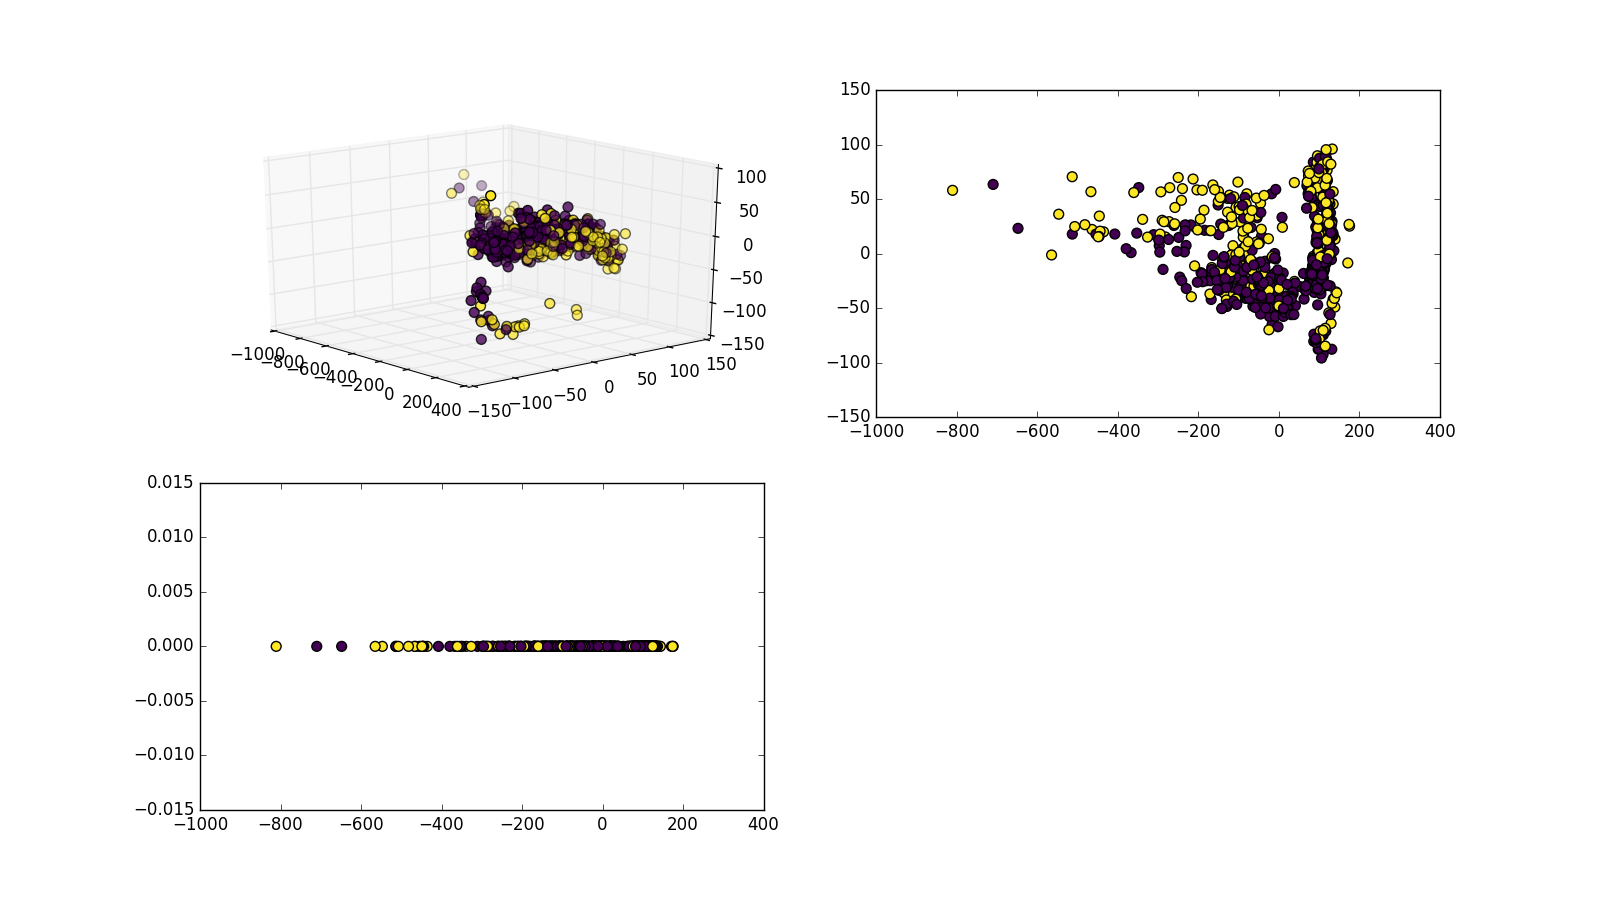
\includegraphics[width=.85\linewidth]{img/experiments/iso_diabetes}
	\captionsetup{justification=centering}
	\caption{The Diabetes data set and its reduction to 3, 2 and 1 dimensions, respectively.}
	\label{fig:iso_diabetes}
\end{figure}

\begin{table}[H]
	\centering
	\begin{tabular}{|c|c|c|c|c|c|}
		\hline
		& \textbf{Orig. ($\mathbb{R}^{8}$}) & \textbf{$\mathbb{R}^{6}$} & \textbf{$\mathbb{R}^{4}$} & \textbf{$\mathbb{R}^{2}$} & \textbf{$\mathbb{R}$} \\\hline
		\textbf{Pred. accuracy}   & .7239 & .7174 & .7252 & .7148 & .6588 \\\hline
		\textbf{GridSearch time}   & .79 s & .94 s & .58 s & .99 s & 7.4 s \\\hline
		\textbf{Reduction time}    & - & 23.55 s & 24.38 s & 26.5 s & 23.44 s \\\hline
		\textbf{Stress} & - & .2875 & .2362 & .3001 & .4462 \\\hline
		\textbf{Data size}  & 48 KB & 36 KB & 24 KB & 12 KB & 6 KB \\\hline
	\end{tabular}
	\captionsetup{justification=centering}
	\caption{Description of predictions and reduction performance for Diabetes data set.}
\end{table}
